\documentclass[12pt,a4paper]{article}
\usepackage[latin1]{inputenc}
\usepackage{amsmath}
\usepackage{amsfonts}
\usepackage{amssymb}
\usepackage{graphicx}
\usepackage{scrlayer-scrpage}
\usepackage[xcdraw]{xcolor}
\usepackage{placeins}
\usepackage{slashbox}
\usepackage{colortbl}
\usepackage{pdfpages}
\usepackage[colorlinks, citecolor=red, linkcolor=blue]{hyperref}
\usepackage{geometry}
\geometry{right=25mm, left=25mm}
\usepackage{caption}

%\usepackage{natbib}

\bibliographystyle{apalike}

%\setcounter{section}{-1}
\arrayrulewidth=1pt

\pagestyle{scrheadings}
\clearpairofpagestyles

\ihead{Andreas Mast}
\chead{Support Bracket Analysis}
\ohead{
\includegraphics[width=2cm]{Bilder/logo.jpg}}
%\ifoot{Fu�zeile innen}
\cfoot[\pagemark]{\pagemark}
%\ofoot{Fu�zeile au�en}

\renewcommand{\baselinestretch}{1.5}


%%%%%%%%%%%%%%%%%%%%%%%%%%%%%%%%%%%%%%%%%%%%%%%%%%%%%%%%%%%%%%%%%%%%%%%
% --Discussion anpassen, Wasserverlust und Kebabwechsel beim Ofen
% --Lineare Anpassung statt Logarithmischer Anpassung
%%%%%%%%%%%%%%%%%%%%%%%%%%%%%%%%%%%%%%%%%%%%%%%%%%%%%%%%%%%%%%%%%%%%%%%



%%%%%
% Start of the document
%%%%%

\begin{document}
	\pagenumbering{Roman}
	
	\begin{titlepage}
		\begin{center}
			
\includegraphics[scale=0.5]{Bilder/logo.jpg}
		\end{center}
		\vspace{1cm}
		\begin{center}
			{\huge Faculty of Computing, Engineering \& Science}	
		\end{center}
		\begin{center}
			{\Large Support Bracket Analysis}
		\end{center}
		\begin{center}
			{\Large \today}
		\end{center}
%		\vspace{1cm}
		\begin{center}
%			\includegraphics[scale=0.7]{Bilder/Oven.png}
		\end{center}
%		\begin{center}
%			{\huge $4^{th}$ March 2018}			
%		\end{center}
%		\vspace{1cm}
		\begin{center}
			\begin{large}
				Andreas Mast - 17158885 
				
				mastandr@hs-albsig.de
			\end{large}
		\end{center}

	\end{titlepage}
	
	\newpage
	\pagenumbering{gobble}
	\tableofcontents
	
	\newpage
	\pagenumbering{gobble}
	
	\pagenumbering{arabic}
 	
	\section{Introduction}
	%allgemeine Einleitung%
	Support brackets are omnipresent and decisive for many construction, even if many people are not aware of them. As the name implies they support crucial parts of a constructions by holding a weight or by holding two parts together. 
	
	%Problem beschreibung%
	In this paper a support bracket with a specific load is investigated. 
	%Bild einf�gen%
	\begin{center}
		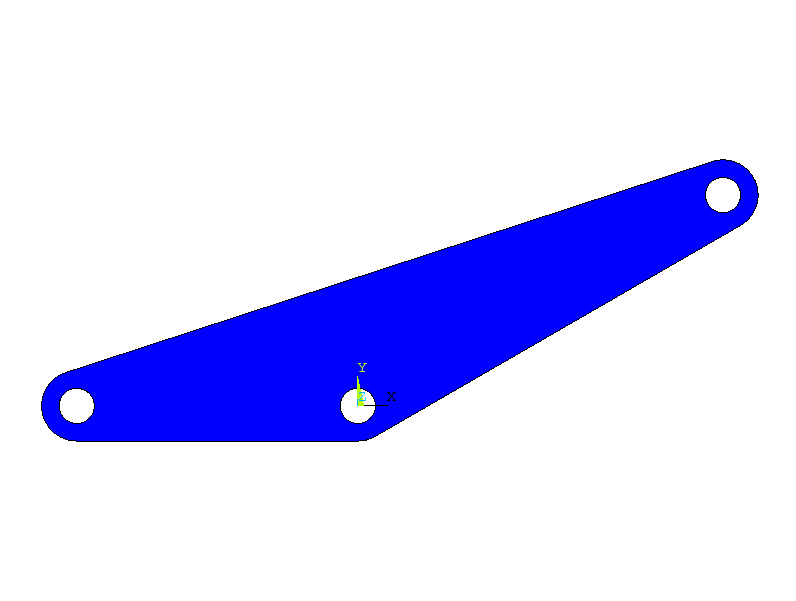
\includegraphics[scale=0.5]{Bilder/1.png}
	\end{center}
	
	%Grund der Analyse%
	The intention of this research is to determine, whether the internal stresses cause a plastic deformation.
	
	%verwendete Software erw�hnen
		
	
	\section{Assumptions}
	
	\begin{enumerate}
		\item static
		\item homogeneous material
		\item isotropic material
		\item Linear elastic
		\item two dimensional
		\item plane stress (small thickness)
		\item weight can be ignored (no gravity)
		\item Evenly distributed load (1885 N at each point)
		\item Friction is ignored
		\item Axle/Pins are rigid
		\item Pins/Axle fits perfectly in holes
	\end{enumerate}

	\section{Modelling the analysis}
	
	\section{Results}
	
	\section{Discussion}
	
	\section{Conclusion}
	

	\bibliography{bib}
\end{document}


